\documentclass[border=12pt]{standalone}
\usepackage{tikz}
\usepackage{amsmath}
\usepackage[T1]{fontenc}
\usepackage{lmodern}
\usetikzlibrary{arrows.meta,positioning,shapes.geometric,calc,fit,backgrounds}

\definecolor{cAgent}{HTML}{2D5BA3}
\definecolor{cAgentBg}{HTML}{E8EFF9}
\definecolor{cChat}{HTML}{1F8A8A}
\definecolor{cChatBg}{HTML}{E2F2F1}
\definecolor{cMgr}{HTML}{8E3A8E}
\definecolor{cMgrBg}{HTML}{F1E5F1}
\definecolor{cArt}{HTML}{B5651D}
\definecolor{cArtBg}{HTML}{FBEFDF}
\definecolor{cSpecBg}{HTML}{EFEFEF}
\definecolor{cInk}{HTML}{2A2A2A}
\definecolor{cP1}{HTML}{4A6FA0}
\definecolor{cP2}{HTML}{9B5A91}

\begin{document}

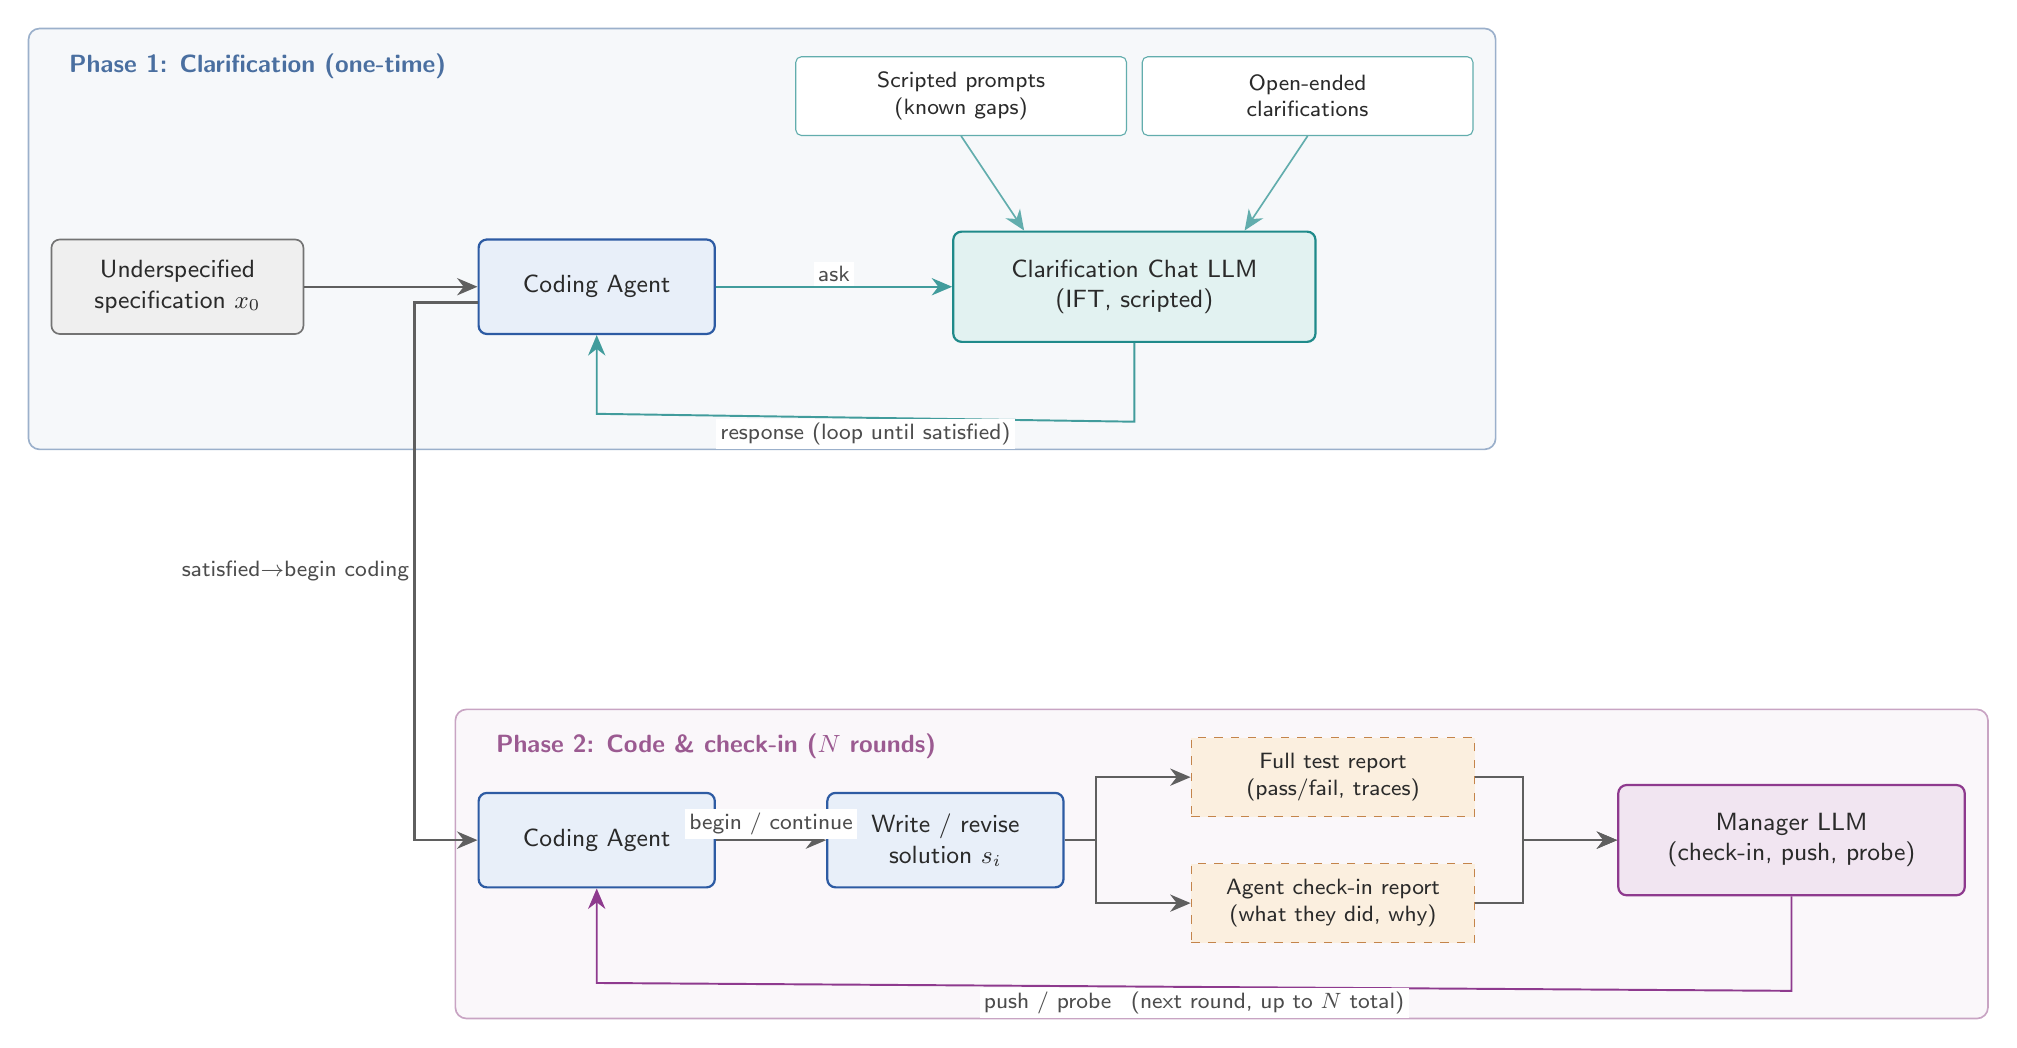
\begin{tikzpicture}[
    font=\sffamily\small,
    >={Stealth[length=2.6mm,width=2.2mm]},
    every node/.style={text=cInk},
    every path/.style={line width=0.55pt, draw=cInk!75},
    spec/.style={
        rectangle, rounded corners=3pt, draw=black!55, line width=0.6pt,
        fill=cSpecBg, minimum width=32mm, minimum height=12mm,
        align=center, inner sep=4pt
    },
    agent/.style={
        rectangle, rounded corners=3pt, draw=cAgent, line width=0.8pt,
        fill=cAgentBg, minimum width=30mm, minimum height=12mm,
        align=center, inner sep=4pt
    },
    chat/.style={
        rectangle, rounded corners=3pt, draw=cChat, line width=0.8pt,
        fill=cChatBg, minimum width=46mm, minimum height=14mm,
        align=center, inner sep=4pt
    },
    manager/.style={
        rectangle, rounded corners=3pt, draw=cMgr, line width=0.8pt,
        fill=cMgrBg, minimum width=44mm, minimum height=14mm,
        align=center, inner sep=4pt
    },
    artifact/.style={
        rectangle, draw=cArt!80, line width=0.5pt, dashed,
        fill=cArtBg, minimum width=36mm, minimum height=10mm,
        align=center, inner sep=3pt, font=\sffamily\footnotesize
    },
    mode/.style={
        rectangle, rounded corners=2pt, draw=cChat!70, line width=0.4pt,
        fill=white, minimum width=42mm, minimum height=10mm,
        align=center, inner sep=4pt, font=\sffamily\footnotesize
    },
    phaselbl/.style={font=\sffamily\bfseries\small},
    grouplabel/.style={font=\sffamily\footnotesize\itshape, text=black!55},
    flow/.style={->, line width=0.6pt, draw=cInk!75},
    flowmgr/.style={->, line width=0.7pt, draw=cMgr},
    flowchat/.style={->, line width=0.7pt, draw=cChat!85},
    edgelbl/.style={font=\sffamily\footnotesize, fill=white, inner sep=1.5pt, text=black!70},
]

% =====================================================
% Phase 1 row
% =====================================================

\node[spec] (spec) {Underspecified\\specification $x_0$};
\node[agent, right=22mm of spec] (agent1) {Coding Agent};
\node[chat,  right=30mm of agent1] (chat)   {Clarification Chat LLM\\(IFT, scripted)};

% modes above chat
\node[mode, above=12mm of chat, xshift=-22mm] (script) {Scripted prompts\\(known gaps)};
\node[mode, above=12mm of chat, xshift=22mm]  (open)   {Open-ended\\clarifications};

% phase 1 forward edges
\draw[flow] (spec) -- (agent1);
\draw[flowchat] (agent1) -- node[edgelbl, above]{ask} (chat);
\draw[flow, draw=cChat!70] (script.south) -- ($(chat.north)+(-14mm,0)$);
\draw[flow, draw=cChat!70] (open.south)   -- ($(chat.north)+(14mm,0)$);

% Channel anchors (invisible) inside phase 1 to route the loop
\coordinate (p1loopL) at ($(agent1.south)+(0,-10mm)$);
\coordinate (p1loopR) at ($(chat.south)+(0,-10mm)$);

% chat -> agent response (right-angle, inside panel via channel)
\draw[flowchat]
    (chat.south) -- (p1loopR)
    -- node[edgelbl, below, pos=0.5]{response (loop until satisfied)} (p1loopL)
    -- (agent1.south);

% =====================================================
% Phase 2 row
% =====================================================

\node[agent,    below=58mm of agent1] (agent2)     {Coding Agent};
\node[agent,    right=14mm of agent2] (code)       {Write / revise\\solution $s_i$};
\node[artifact, right=16mm of code, yshift=8mm]   (tests)      {Full test report\\(pass/fail, traces)};
\node[artifact, right=16mm of code, yshift=-8mm]  (selfreport) {Agent check-in report\\(what they did, why)};
\node[manager,  right=18mm of tests, yshift=-8mm] (mgr)        {Manager LLM\\(check-in, push, probe)};

% phase 2 forward edges
\draw[flow] (agent2) -- node[edgelbl, above]{begin / continue} (code);
\draw[flow] (code.east) -- ++(4mm,0) |- (tests.west);
\draw[flow] (code.east) -- ++(4mm,0) |- (selfreport.west);
\draw[flow] (tests.east)      -- ++(6mm,0) |- (mgr.west);
\draw[flow] (selfreport.east) -- ++(6mm,0) |- (mgr.west);

% Channel anchors inside phase 2
\coordinate (p2loopL) at ($(agent2.south)+(0,-12mm)$);
\coordinate (p2loopR) at ($(mgr.south)+(0,-12mm)$);

% manager -> agent2 (right-angle, inside panel)
\draw[flowmgr]
    (mgr.south) -- (p2loopR)
    -- node[edgelbl, below, pos=0.5]{push / probe \, (next round, up to $N$ total)} (p2loopL)
    -- (agent2.south);

% =====================================================
% Transition Phase 1 -> Phase 2
% =====================================================

% Drop down from the left edge of agent1 (away from the chat loop on the right)
\draw[flow, line width=0.8pt]
    ($(agent1.west)+(0,-2mm)$) -- ++(-8mm,0)
    |- node[edgelbl, pos=0.25, left]{satisfied$\rightarrow$\\begin coding}
    (agent2.west);

% =====================================================
% Background phase panels (include channel coords in fit)
% =====================================================

\begin{scope}[on background layer]
    \node[draw=cP1!55, line width=0.6pt, rounded corners=4pt, fill=cP1!5,
          fit=(spec)(agent1)(chat)(script)(open)(p1loopL)(p1loopR),
          inner sep=8pt, inner ysep=10pt] (p1box) {};
    \node[phaselbl, text=cP1, anchor=north west, xshift=4mm, yshift=-2mm]
          at (p1box.north west) {Phase 1: Clarification (one-time)};
\end{scope}

\begin{scope}[on background layer]
    \node[draw=cP2!55, line width=0.6pt, rounded corners=4pt, fill=cP2!5,
          fit=(agent2)(code)(tests)(selfreport)(mgr)(p2loopL)(p2loopR),
          inner sep=8pt, inner ysep=10pt] (p2box) {};
    \node[phaselbl, text=cP2, anchor=north west, xshift=4mm, yshift=-2mm]
          at (p2box.north west) {Phase 2: Code \& check-in ($N$ rounds)};
\end{scope}

\end{tikzpicture}

\end{document}
